\begin{task}{2, Simulation of the scenario with a different model}
Once we have tested Vadere's default model, Optimal Steps Model, we can try to experiment with other models, like the Social Force Model.

After testing this new model in RiMEA 1 and the chicken test, we can observe there is almost no changes in the pedestrian behaviour, the pedestrians travel to the goal as before. Figure \ref{rimeachickensfm}a and Figure \ref{rimea1}a seem to be exactly equal. In the chicken test (Figure \ref{rimeachickensfm}b), the only difference, barely perceptible, is the path each model takes in the first steps out of the obstacle structure. The OSM model faces the obstacles until it dodges them, while the SFM feels the disturbance of the obstacles from the start and takes a slightly more diagonal initial path. A priori, this may indicate that a difference between the two models lie in the repulsive potential function of the obstacles.

\begin{figure}[H] 
\centering
\subfigure[RiMEA 1]{
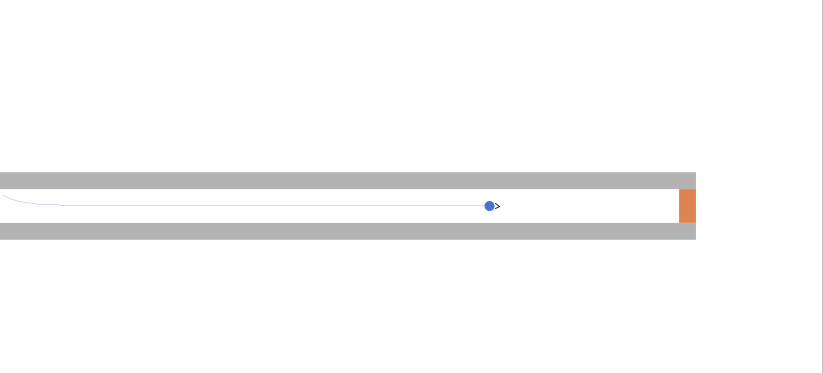
\includegraphics[scale=0.35]{report-template/images/rimea1_social.png}}
\subfigure[Chickent test]{
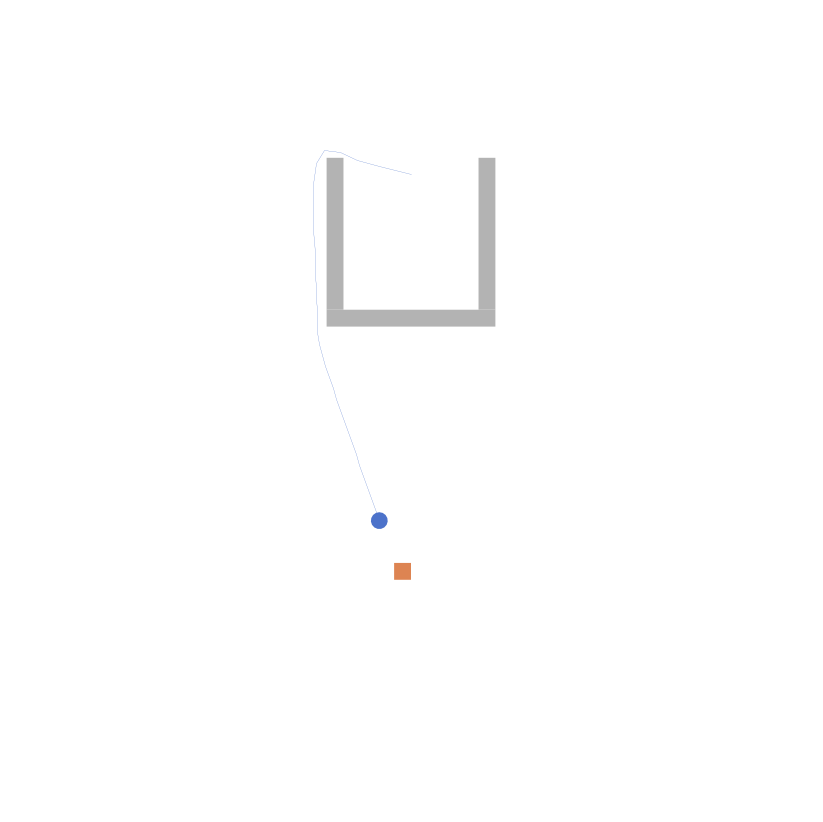
\includegraphics[scale=0.35]{report-template/images/chicken_social.png}}
\caption{RiMEA 1 and chicken test with SFM}
\label{rimeachickensfm}
\end{figure}

By definition, RiMEA 6 requires obstacle avoidance as well as pedestrian avoidance in both models. Therefore, now we can observe more differences than before testing on this scenario.

As we hypothesised with the chicken test, it now seems clear that both models have different functions for modelling pedestrian repulsion to obstacles and to other pedestrians. Looking at the critical point which is the corner of the scenario, we can see how the pedestrians are positioned in the two models. In OSM they have more distance between them and there is less density of pedestrians in the corner, being able to move away from the wall. However, in SFM the pedestrians stick close together, going almost completely in a line during the final corridor. That is, in SFM every pedestrian seems to follow exactly the same path as we can observe in Figure \ref{rimea6sfm}d.

\begin{figure}[H] 
\centering
\subfigure[RiMEA 6 OSM corner]{
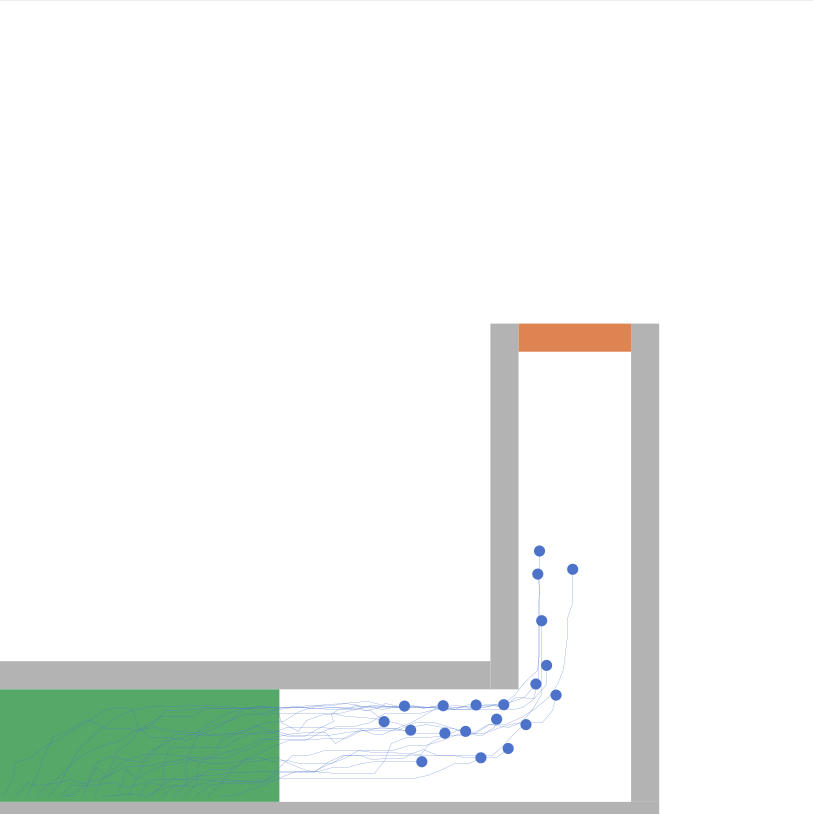
\includegraphics[scale=0.35]{report-template/images/rimea6_optimal_middle.png}}
\subfigure[RiMEA 6 SFM corner]{
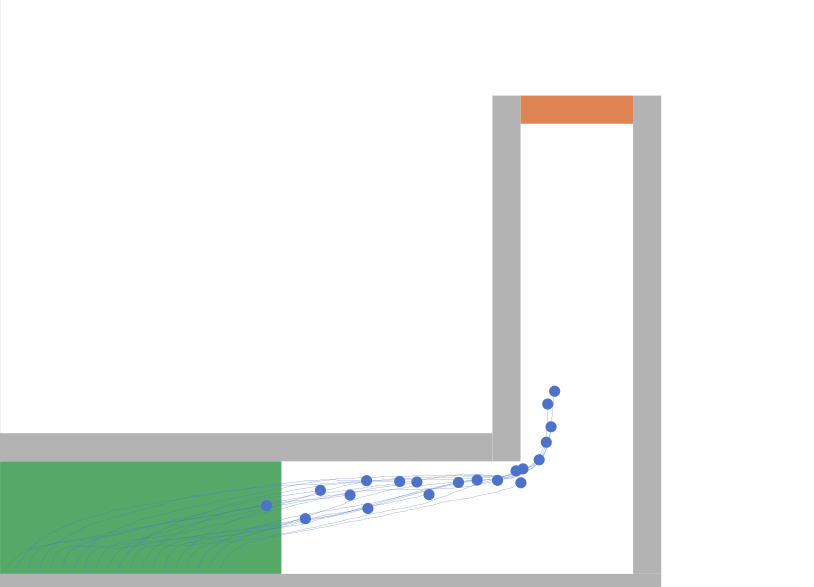
\includegraphics[scale=0.35]{report-template/images/rimea6_social_middle.png}}
\subfigure[RiMEA 6 OSM finished]{
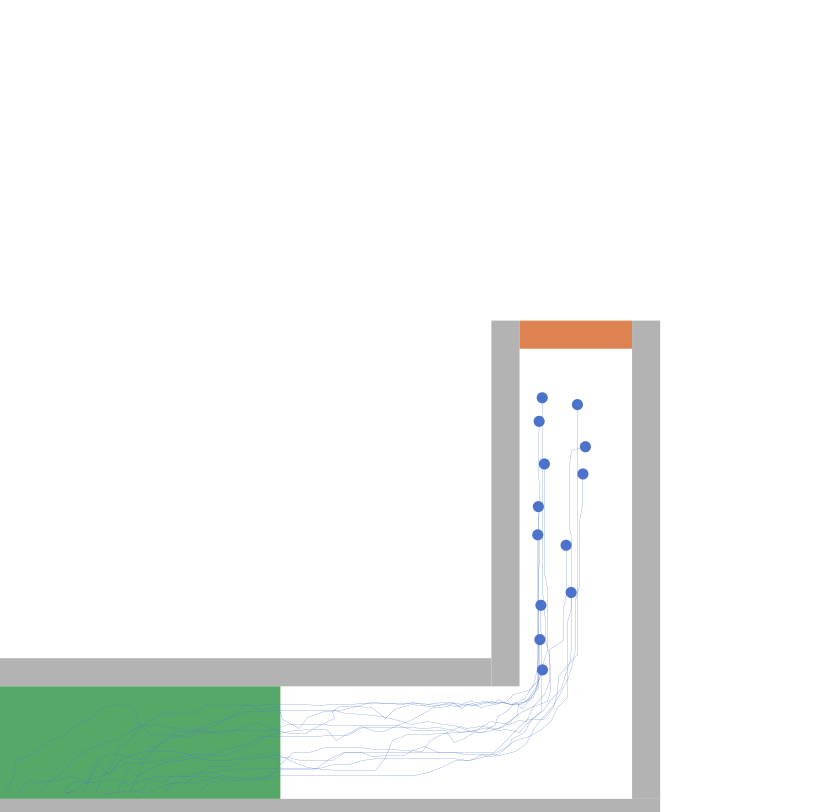
\includegraphics[scale=0.35]{report-template/images/rimea6_optimal_finish.png}}
\subfigure[RiMEA 6 SFM finished]{
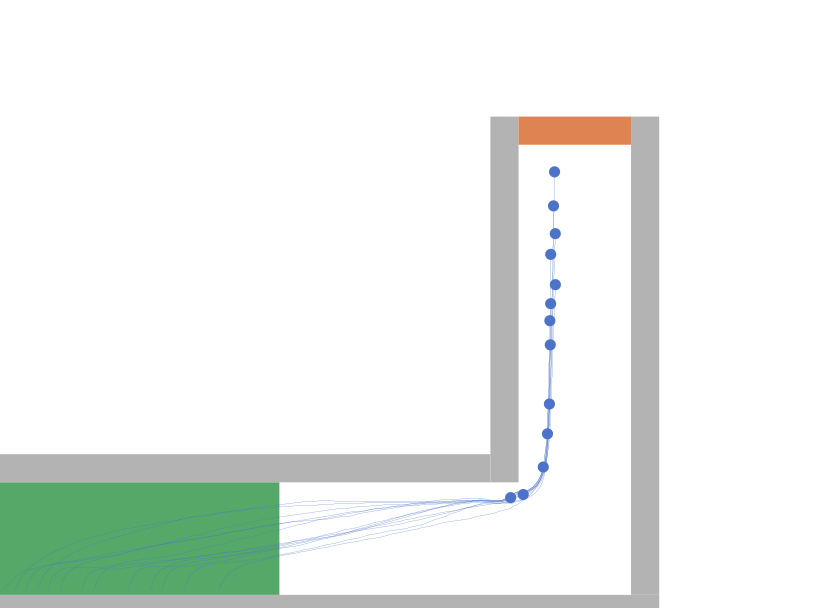
\includegraphics[scale=0.35]{report-template/images/rimea6_social_finish.png}}
\caption{Comparison between SFM and OSM in RiMEA 6}
\label{rimea6sfm}
\end{figure}

As it is said in Ref \cite{helbing1995social}, the SFM's pedestrian movement is mainly computed taking into account the motivation of a pedestrian to accelerate or decelerate, depending on the external forces that surround it. These external forces are mainly: The shortest way to reach the goal given a desired speed, the pedestrians near itself, the obstacles near it and the possibility that a pedestrian is attracted by other persons (friends, celebrity, etc.). Also, it is important to note that this model gives weaker influence to situations located behind a pedestrian, coherent when observing the organization of pedestrians in Figure \ref{rimea6sfm}d where they follow each other. SFM uses differential equations to model all these interactions. 

On the other hand, the OSM model's pedestrian use discrete movement in a continuous space, taking into account a floor field where pedestrians and obstacles have repulsive potential \cite{seitz2012natural}. 

Therefore, the main differences between the behaviour of the two models, apart from their own way of defining the function that models the repulsion of obstacles and other pedestrians, is that in the case of OSM, the pedestrians have a discrete motion, which makes them move more like real people and not like particles. This can be realized in Figure \ref{rimea6sfm}a, where the OSM model got a more realistic approach of how a crowd would distribute itself around a corner.

In addition, OSM's pedestrians, as stated in \cite{seitz2012natural}, can decide whether to move closer to their desired speed, slow down or maintain a group structure, whereas SFM's pedestrians move accelerated by external forces, one of them being arriving at the goal using the shortest path. This difference can be noted in Figure \ref{rimea6sfm}c and Figure \ref{rimea6sfm}d.


After testing and comparing OSM and SFM models, we tried the Gradient Navigation Model. Without reading its related publication, we can already observe that this model tries to take the most optimal way to the goal, being very tolerant of being close to obstacles. We can observe in Figure \ref{rimeachickengnm}a the pedestrian does not initially position itself in the centre, like the previous models did, in order to be separated from obstacles, but takes the fastest way, going straightforward directly. Also, we can see how in Figure \ref{rimeachickengnm}b the pedestrian takes the path closest to the obstacles, being this the shortest one.


\begin{figure}[H] 
\centering
\subfigure[RiMEA 1]{
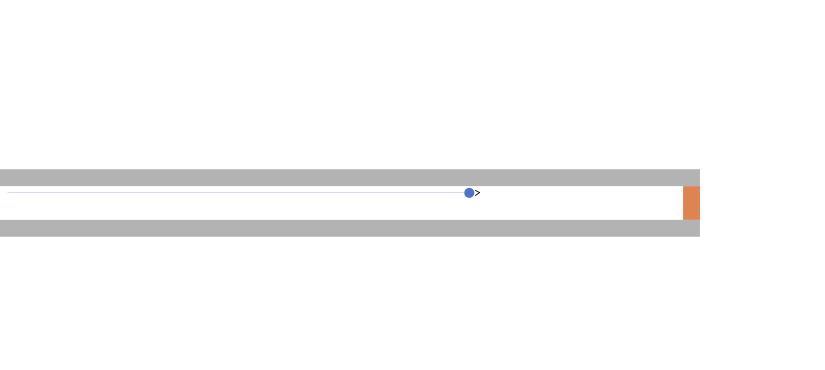
\includegraphics[scale=0.35]{report-template/images/rimea1_gradient.png}}
\subfigure[Chickent test]{
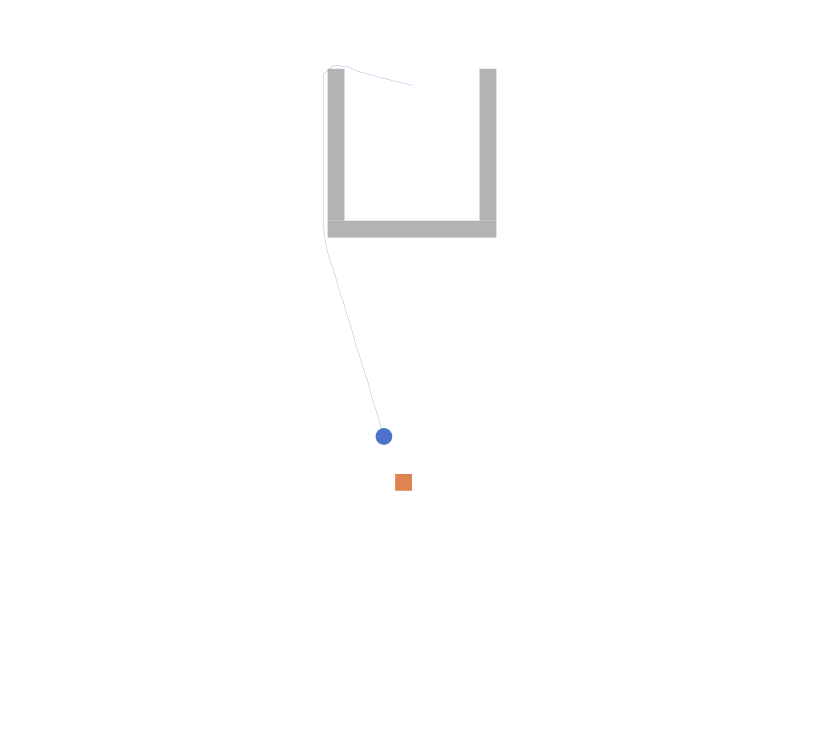
\includegraphics[scale=0.35]{report-template/images/chicken_gradient.png}}
\caption{RiMEA 1 and chicken test with GNM}
\label{rimeachickengnm}
\end{figure}

In RiMEA 6, we can observe how this behavioural pattern remains. Pedestrians wait their turn to turn the corner, keeping as close to the wall as possible to ensure the most optimal path to the goal.

\begin{figure}[H] 
\centering
\subfigure[RiMEA 6 start]{
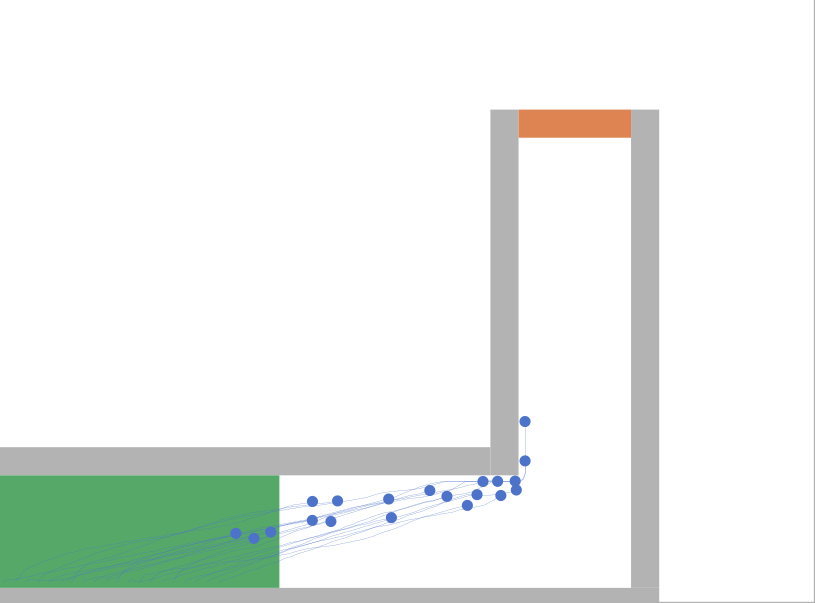
\includegraphics[scale=0.35]{report-template/images/rimea6_gradient_start.png}}
\subfigure[RiMEA 6 middle]{
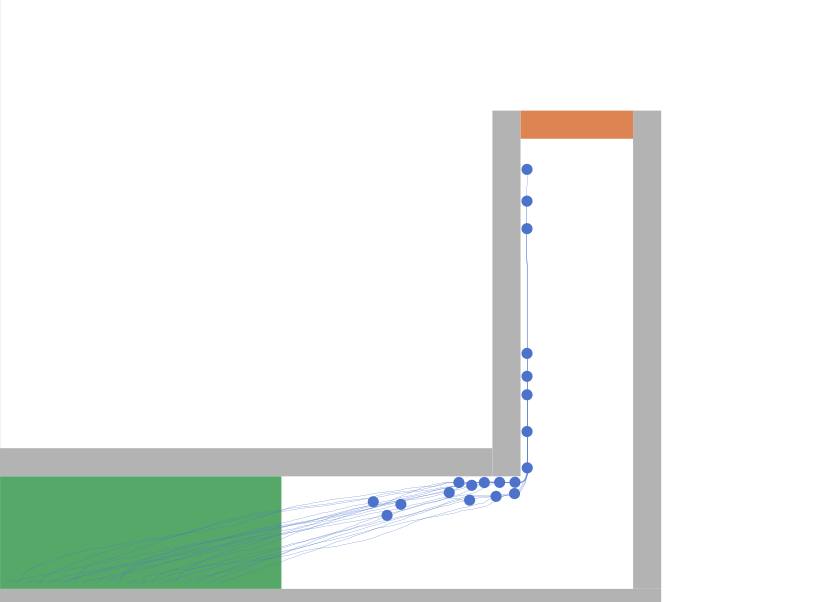
\includegraphics[scale=0.35]{report-template/images/rimea6_gradient_middle.png}}
\subfigure[RiMEA 6 finish]{
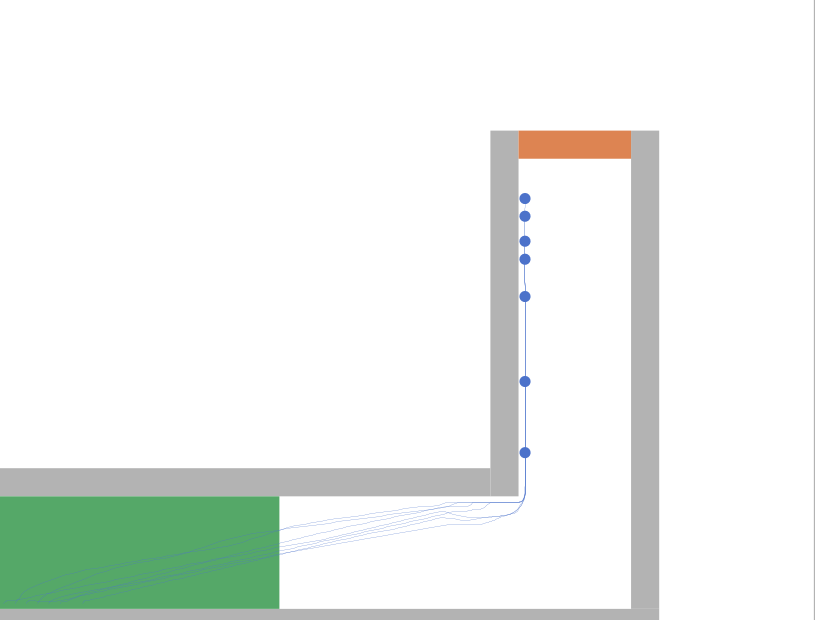
\includegraphics[scale=0.35]{report-template/images/rimea6_gradient_finish.png}}
\caption{RiMEA 6 test with GNM}
\label{rimea6gnm}
\end{figure}

GNM is based on certain assumptions about people's behaviour, like: "Crowd behavior in normal situations is governed by the decisions of the
individuals rather than by physical, interpersonal contact forces" that contrast with the functioning of SFM, where pedestrian acts as if it would be subject to external forces \cite{dietrich2014gradient}. However, if we analyse the publication further, we can better understand the nature of the different functioning of this model. It states that pedestrians want to reach the target in as little time as possible, as SFM also does, and that pedestrians are able to change their desired velocity as a reaction to the presence of pedestrians and obstacles, like OSM. 

Nevertheless, we consider that what causes this distinct behaviour is the navigation function or field, since it is in the paths that the pedestrians of this model follow to the goal that differentiates them most from the other two models. The navigation uses the solution $\sigma$, that represents the first arrival times or walking costs in the specified domain, and $G(x)$, the speed function. \cite{dietrich2014gradient} states that if $G(x)=1$ for all $x$, the solution $\sigma$ represents the length of the shortest path to the closest target region. However, to account for the fact that pedestrians cannot get arbitrarily close to obstacles, the wave is slowed down in the immediate vicinity of walls by reducing the speed function $G$. 

Hence, we believe that GNM excels in path optimization due to its utilization of a constant value for $G$ in this case. As a result, the solution $\sigma$ yields the most efficient path. Also, running simulations in RiMEA 6 reveals that pedestrians situated further from the wall move at a higher speed until they gradually adjust their course to adhere to the optimal path, showcasing the reduction of $G$ in the presence of nearby obstacles. Despite the decrease in pedestrian speed, it seems that approaching the wall allows pedestrians to cover less distance in these test scenarios, establishing the proximity to the wall as the optimal path identified by $\sigma$.



Moreover, observing the results of our cellular automaton in Exercise 1, we can observe that they look very similar to GNM's behaviour. As commented in Task 1, our cellular automaton goes straightforward in RiMEA 1, being GNM the only model that does that too. Looking at the chicken test, our cellular automaton and GNM are the only ones that adhere to the wall to ensure the optimal path. Then, comparing RiMEA 6's results, we can realize that the behaviour is very similar, where pedestrians follow the shortest path waiting for the other pedestrians to turn the corner. 



Our cellular automaton was designed to search for the optimal path using fast marching method. Therefore, this similarity gives us a new clue as to how GNM works. As it is reported in \cite{dietrich2014gradient}, GNM also uses fast marching to solve $\sigma$ \cite{sethian1999level}. Thus, we think that is why both models do the same routes and ensure the optimal path.

The .scenario files for this tasks can be found in the scenarios folder and they are named according to the algorithm in use:
\begin{verbatim}
    <scenario_name>_SFM.scenario
    <scenario_name>_GNM.scenario
    <scenario_name>.scenario #(default one, using OSM)
\end{verbatim}
\end{task}